%%%
% set up document type
%%%
\documentclass[12pt]{article}

%%%
% declare all packages
%%%
\usepackage[left=25mm, top=20mm, right=25mm, bottom=30mm,nohead,nofoot]{geometry} 

\usepackage[T2A]{fontenc}
\usepackage[utf8]{inputenc}
\usepackage[english, russian]{babel}

\usepackage{graphics, graphicx}

\usepackage{url}
\usepackage{hyperref}

\usepackage{amssymb,latexsym} 
\usepackage{MnSymbol}
\usepackage{mathrsfs}

\usepackage[nottoc,numbib]{tocbibind}
\usepackage{float}
\usepackage{listings}
\usepackage{multirow}
\usepackage{hhline}

\usepackage{color,colortbl}

%%%
% document settings
%%%
\setcounter{tocdepth}{4}
\graphicspath{ {./pic/} }

\renewcommand{\listoffigures}{\begingroup  % add number to list of graphics
\tocsection
\tocfile{\listfigurename}{lof}
\endgroup}
\renewcommand{\listoftables}{\begingroup  % add number to list of tables
\tocsection
\tocfile{\listtablename}{lot}
\endgroup}

%******************************************************************
%******************************************************************
\begin{document}

\begin{titlepage}
	\center
		Санкт-Петербургский Политехнический 
		университет Петра Великого
		Институт прикладной математики и механики
		\\ \textbf{Кафедра «Прикладная математика»}

	\vfill ~
	\textbf{
		\\ \large ЛАБОРАТОРНАЯ РАБОТА №1
	}
	\\	по дисциплине 
	\\	"Математическая статистика"

	\vfill ~

	Выполнил студент гр. \textbf{33631/1} \\
	\textbf{Лансков.Н.В.} \\ 

\vfill

{\large}	Санкт-Петербург
\\ 2019
\end{titlepage}

%%%
% Table of conetnts 
%%%

\tableofcontents 
\newpage
\listoffigures
\newpage
% \listoftables
% \newpage

%%%
% Text
%%%
\section{Постановка задачи}
Сравнить графики распределения выборок случайных чисел, сгенерированных при помощи различных функций распределения, с теоретическими кривыми распределения для выборок мощностями 10, 50, 100.

\section{Теория}
Рассмотрим использованные распределения подробней. Общий вид распределений можно проверить, например, тут: \cite{wiki}

\subsection{Нормальное распределение}

\begin{equation}
f(x)= \frac{1}{\sqrt{2\pi}}e^{-\frac{x^2}{2}}
\end{equation}

\subsection{Распределение Коши}

\begin{equation}
f(x)= \frac{1}{\pi}\bigg( \frac{1}{x^2 + 1}\ \bigg)
\end{equation}

\subsection{Распределение Лапласа}

\begin{equation} 
f(x)= \frac{1}{\sqrt{2}}e^{-\sqrt{2}x}
\end{equation}

\subsection{Равномерное распределение}

\begin{equation}
      f(x) = 
      \begin{cases}
      \frac{1}{2\sqrt{3}}, \quad |x| \leq \sqrt{3} \\
      0, \qquad |x| > \sqrt{3}
      \end{cases}
\end{equation}

\subsection{Распределение Пуассона}

\begin{equation}
P(7) = \frac{7^k}{k!}e^{-7}
\end{equation}

\pagebreak

\section{Реализация}
Выполнено средствами \textit{python} c применением библиотек \textit{numpy, scipy} and \textit{matplotlib}

\section{Результаты}

\begin{figure}[h!]
\begin{center}
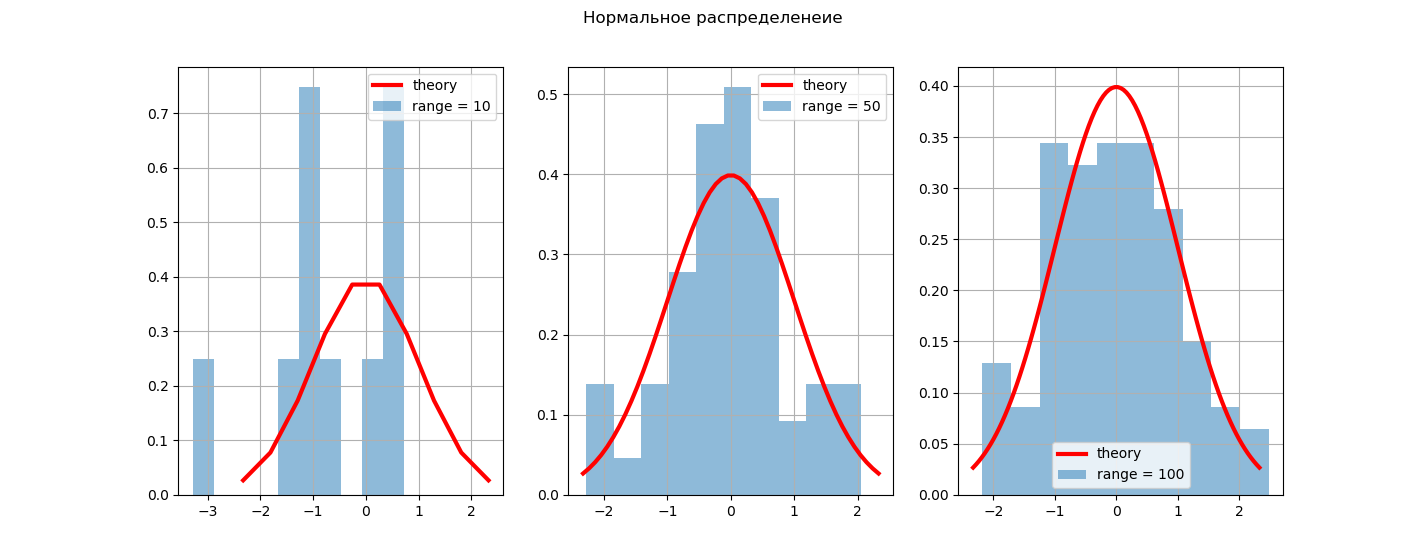
\includegraphics[width=\textwidth]{normal.png} 
\caption{Нормальное распределение}
\end{center}
\end{figure}

\begin{figure}[h!]
\begin{center}
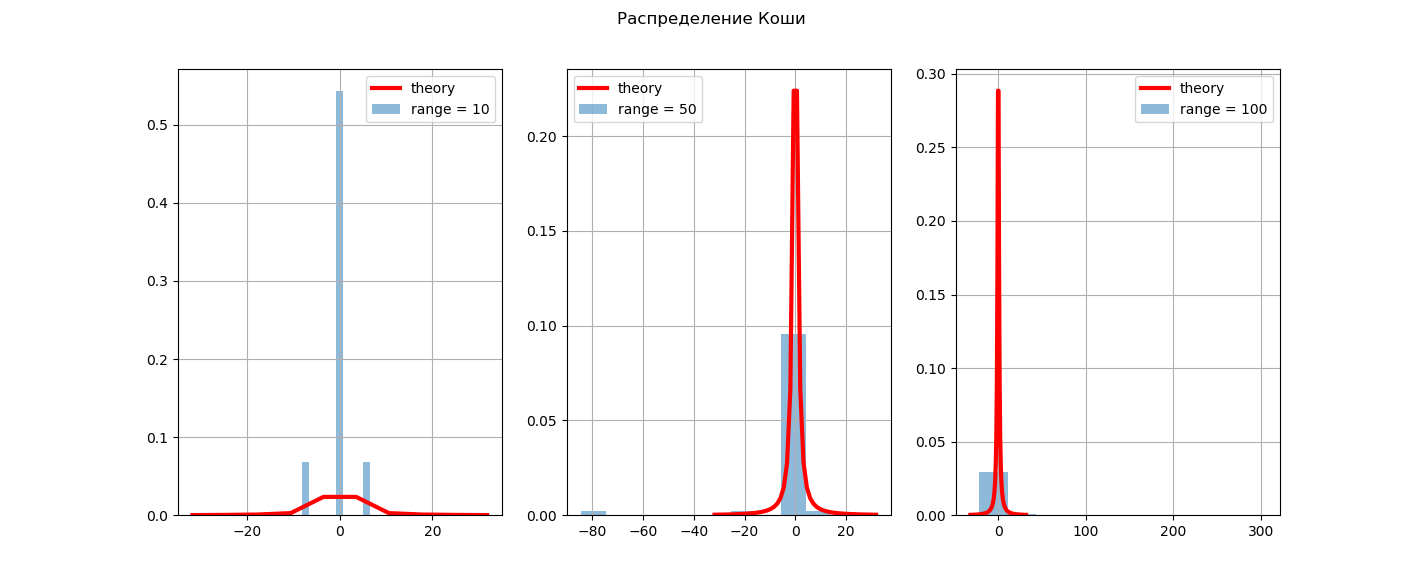
\includegraphics[width=\textwidth]{caushi.png}
\caption{Распределение Коши}
\end{center}
\end{figure}

\pagebreak

\begin{figure}[h!]
\begin{center}
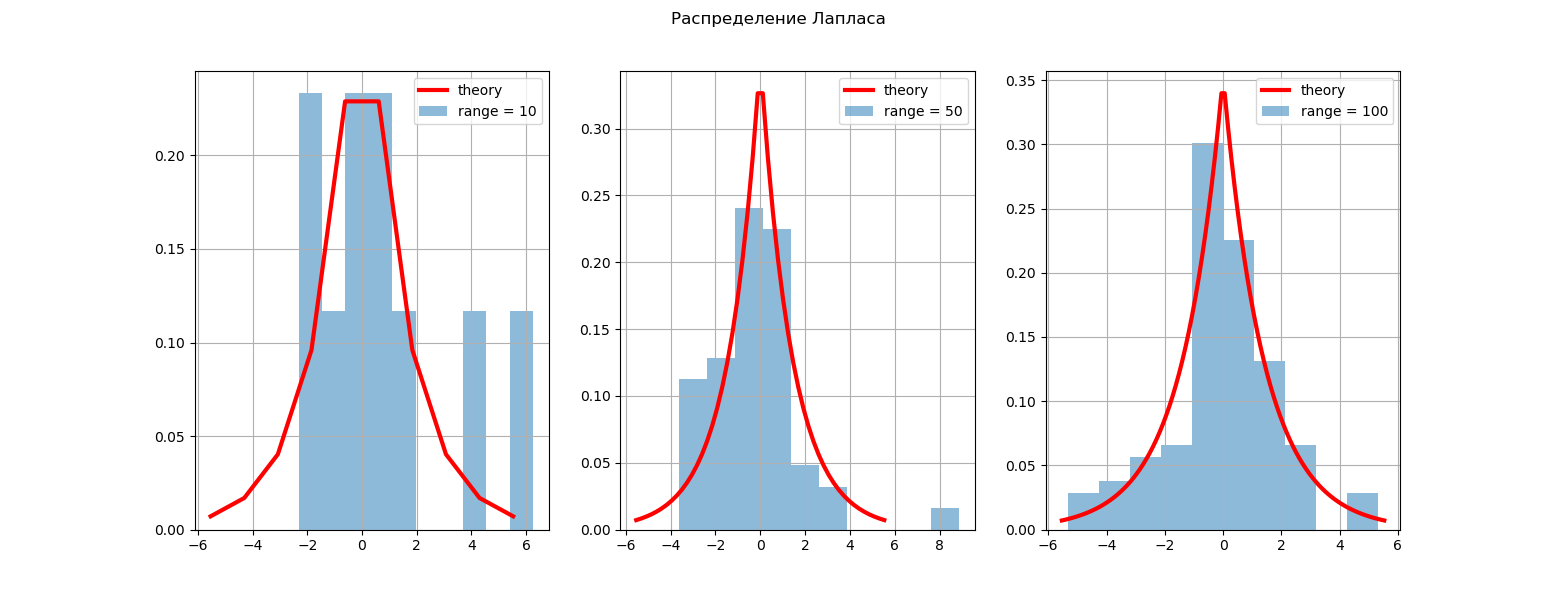
\includegraphics[width=\textwidth]{laplace.png}
\caption{Распределение Лапласа}
\end{center}
\end{figure}

\begin{figure}[h!]
\begin{center}
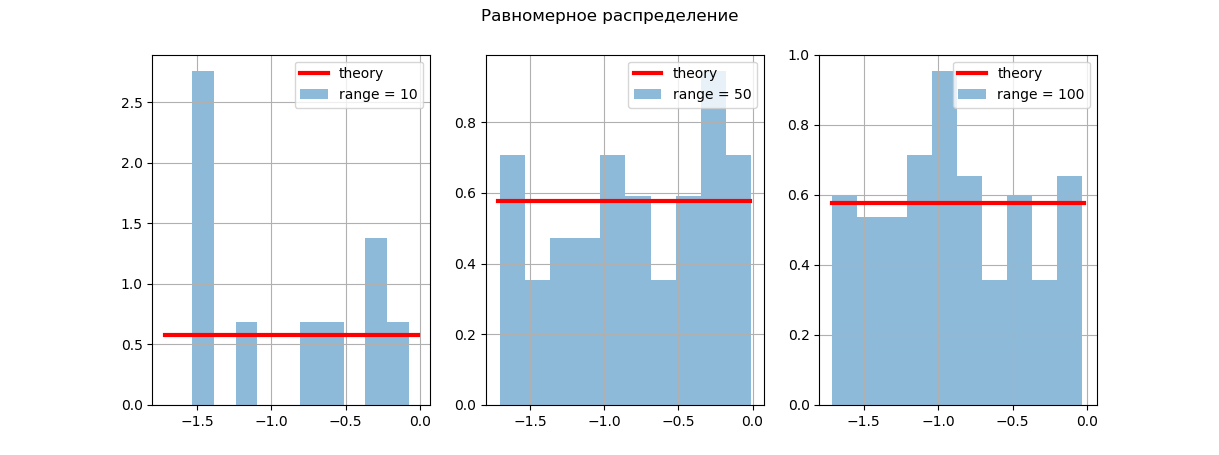
\includegraphics[width=\textwidth]{uniform.png}
\caption{Равномерное распределение}
\end{center}
\end{figure}

\pagebreak

\begin{figure}[h!]
\begin{center}
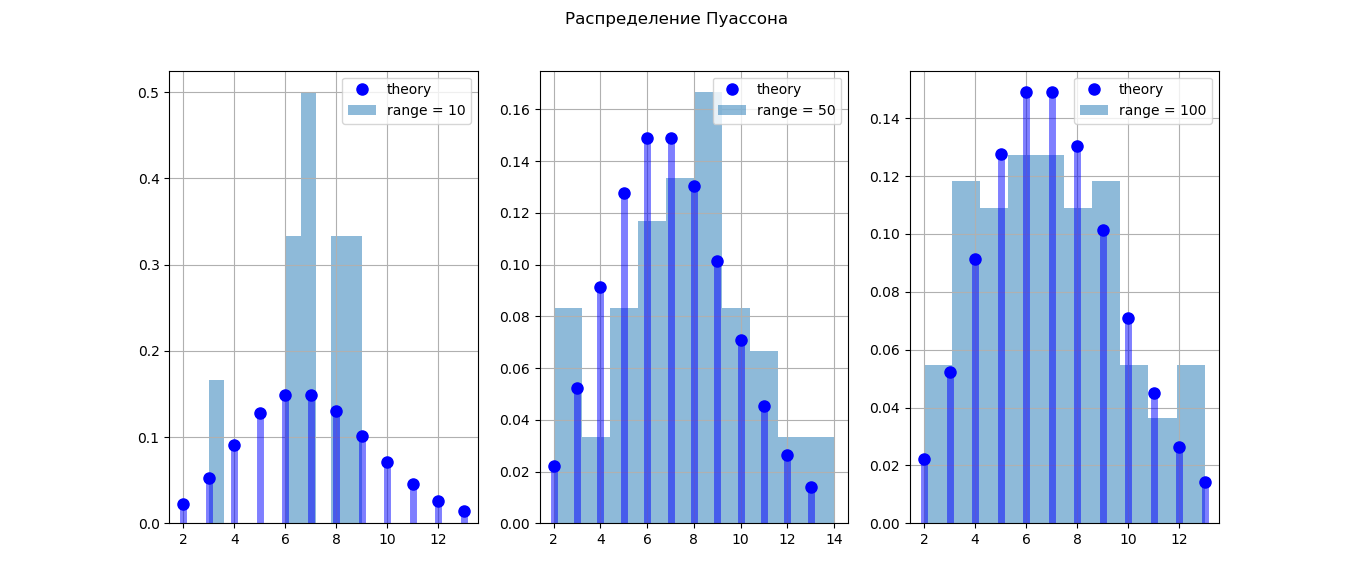
\includegraphics[width=\textwidth]{poisson.png}
\caption{Распределение Пуассона}
\end{center}
\end{figure}

\section{Выводы}

В результате работы были построены графики для трёх выборок разных мощностей для каждого из рассматриваемых распределений. Из графиков видно, что с увеличением мощности выборки, диаграмма всё менее отклоняется от теоретического значения. Это иллюстрирует факт того, что при стремлении можности выборки к бесконечности диаграмма выборки будет оцениваться теоретической кривой с любой интересующей нас точностью.
\par
Конечно, за счёт того что размеры выборок довольно малы, то могут наблюдаться некоторые "выбросы" в конкретных точках (особенно заметно на самых левых графиках для мощности 10). Это объясняется тем, что значения выборки генерируются случайным образом и данных на такой мощности для построения теоретических оценок оказывается недостаточно.

\section{Приложения}

Исходники: \url{https://github.com/LanskovNV/math_statistics/tree/master/lab_1}

%%%
% Literature
%%% 
\begin{thebibliography}{}
    \bibitem{wiki} https://www.wikipedia.org/
\end{thebibliography}

\end{document}